% replace all text with your own text.
% in this template few examples are mention

\chapter{Methodology}

    
\section{Time Series Visualization \& Seasonality Analysis}
The time series decomposition gives key insights into the underlying trend, seasonality and residual components of cocoa prices. The trend line shows a steady increase in cocoa prices over time, with a spike near the end of the period, suggesting the rise in cocoa prices could be attributed to market dynamics, including supply shortages, increasing demand or even external economic factors. The seasonal component exhibits strong periodic fluctuations, potentially corresponding to agricultural cycles, harvest seasons, global demand shifts, or a combination of the three. These oscillations are indicative of the presence of a well-defined seasonal effect in cocoa prices. The remainder component captures fluctuations that can not be explained by trend or seasonality. The residual component maintains stability, matching the trend line decomposition, however, the increase in volatility near the end of the period suggests market instability or an extrinsic shock affecting cocoa prices. \\
\begin{figure}[!ht]
    \centering
    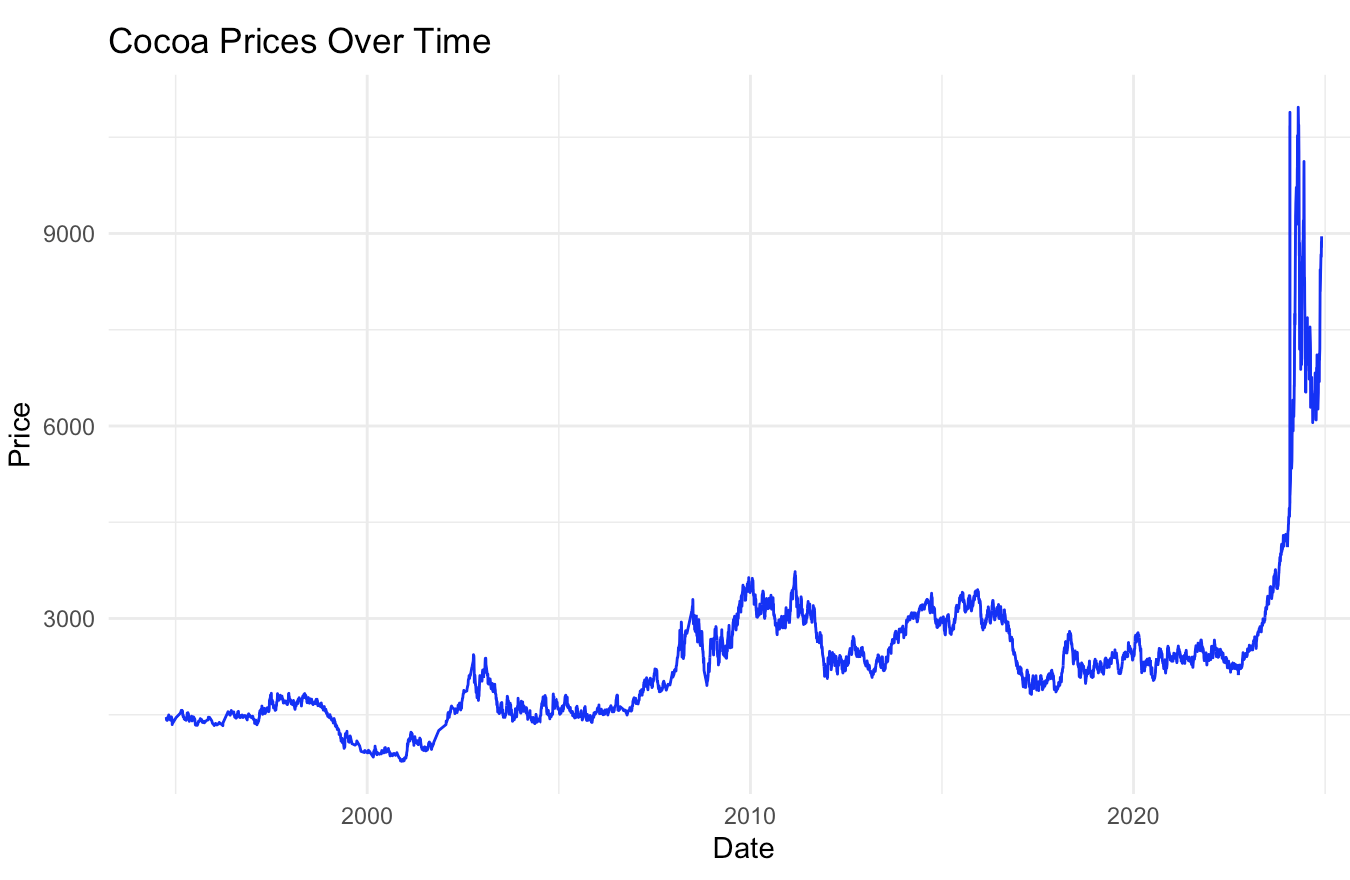
\includegraphics[scale=0.5]{figures/1.1.1.png}
    \caption{Cocoa Prices Over Time}
    \label{fig:chart_a}
\end{figure}

\begin{figure}[!ht]
    \centering
    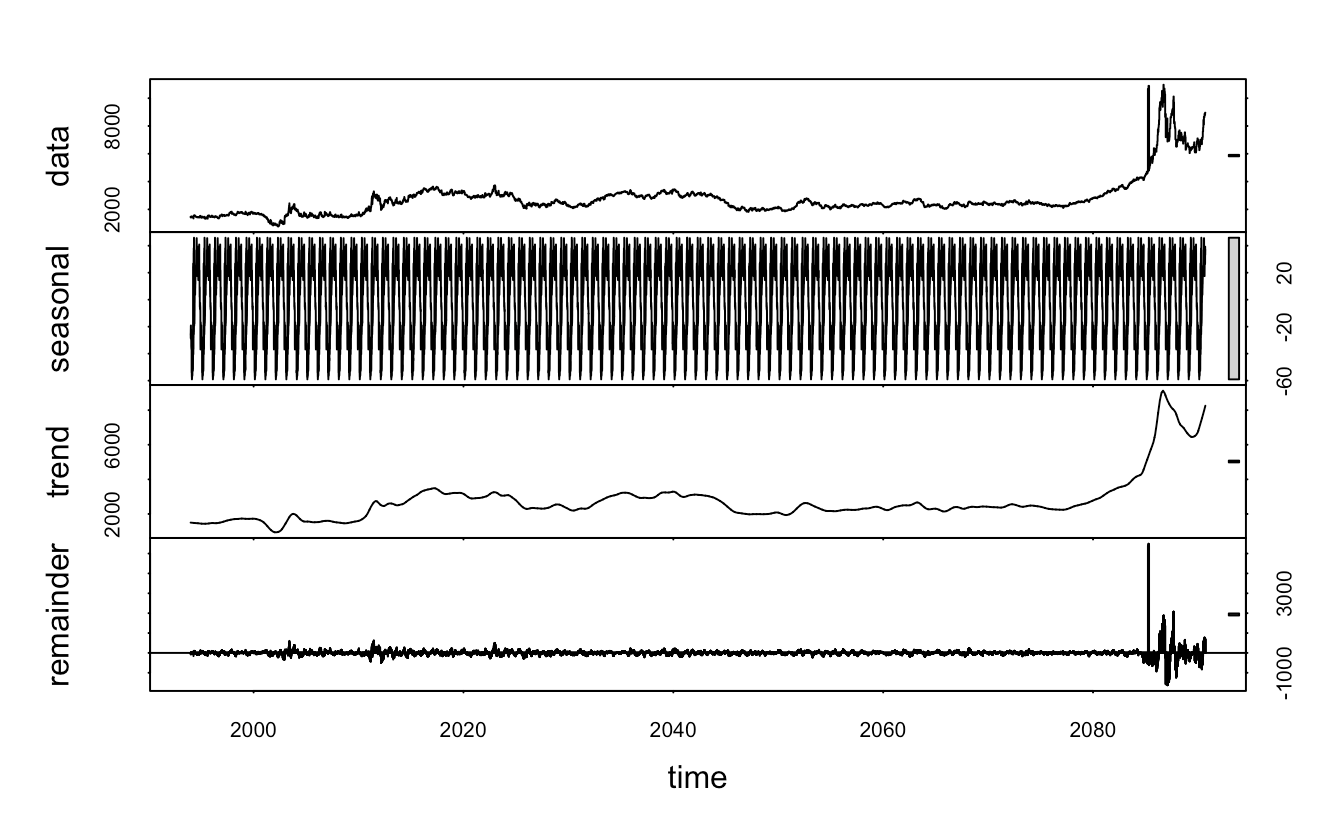
\includegraphics[scale=0.5]{figures/1.1.2.png}
    \caption{Time Series Decomposition of Cocoa Prices}
    \label{fig:chart_a}
\end{figure}

\section{ACF \& PACF Analysis}
Next, we analyze the PACF and ACF of the Cocoa Prices dataset in order to determine an appropriate model. The ACF shows strong persistent autocorrelation at all lags, indicating a strong influence of past cocoa prices on future prices. The ACF suggests that cocoa prices have a strong dependency over time, typical of financial and commodity markets. In contrast, the PACF shows a significant correlation at the first few lags, followed by a sharp drop, suggesting the data may be modelled via an autoregressive process, where the most recent values play a crucial role in predicting future prices. The ACF and PACF suggest and ARIMA model may a suitable choice for forecasting, potentially with an autoregressive component. 

\begin{figure}[!ht]
    \centering
    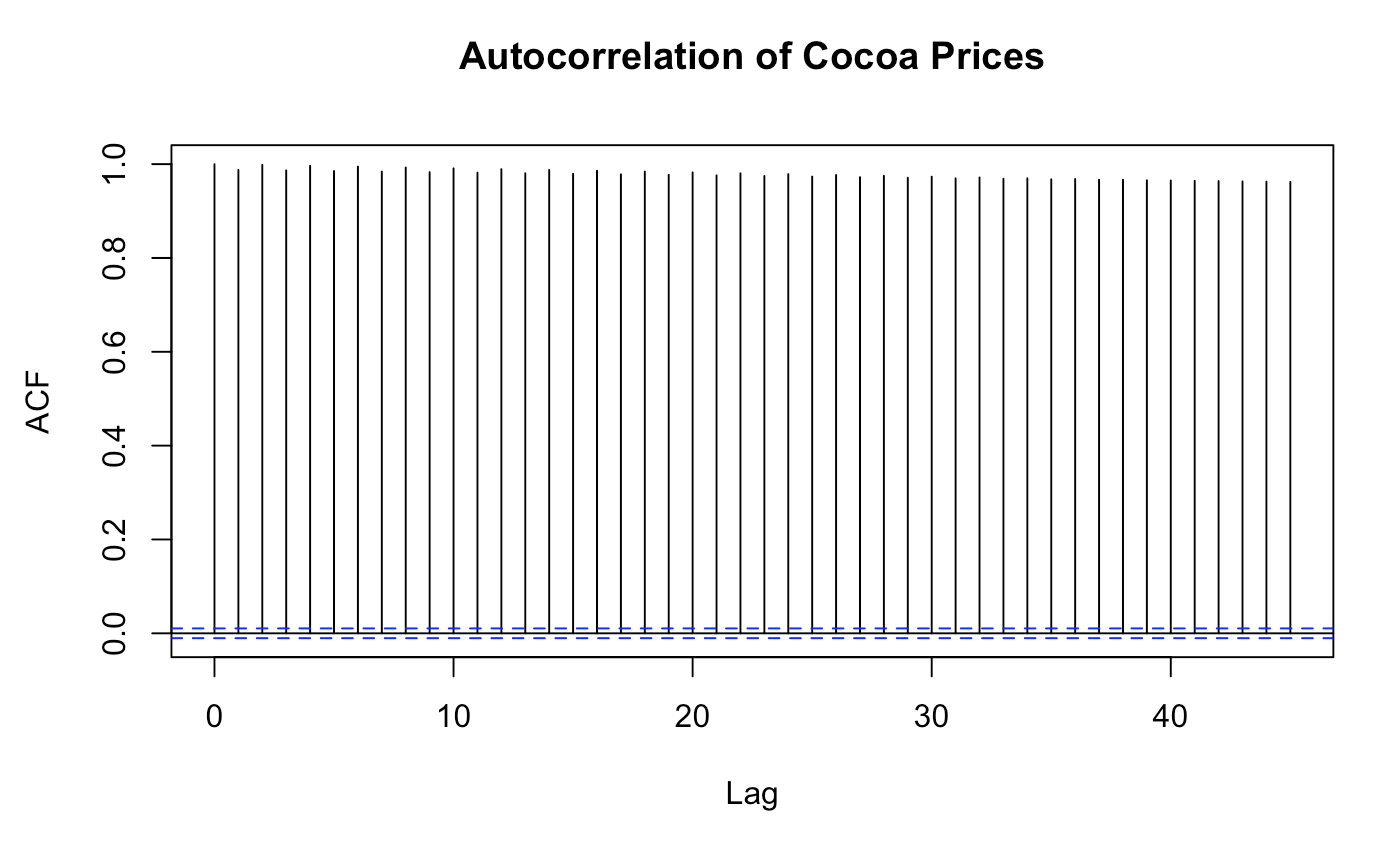
\includegraphics[scale=0.5]{figures/1.1.3.png}
    \caption{ACF of Cocoa Prices}
    \label{fig:chart_a}
\end{figure}

\begin{figure}[!ht]
    \centering
    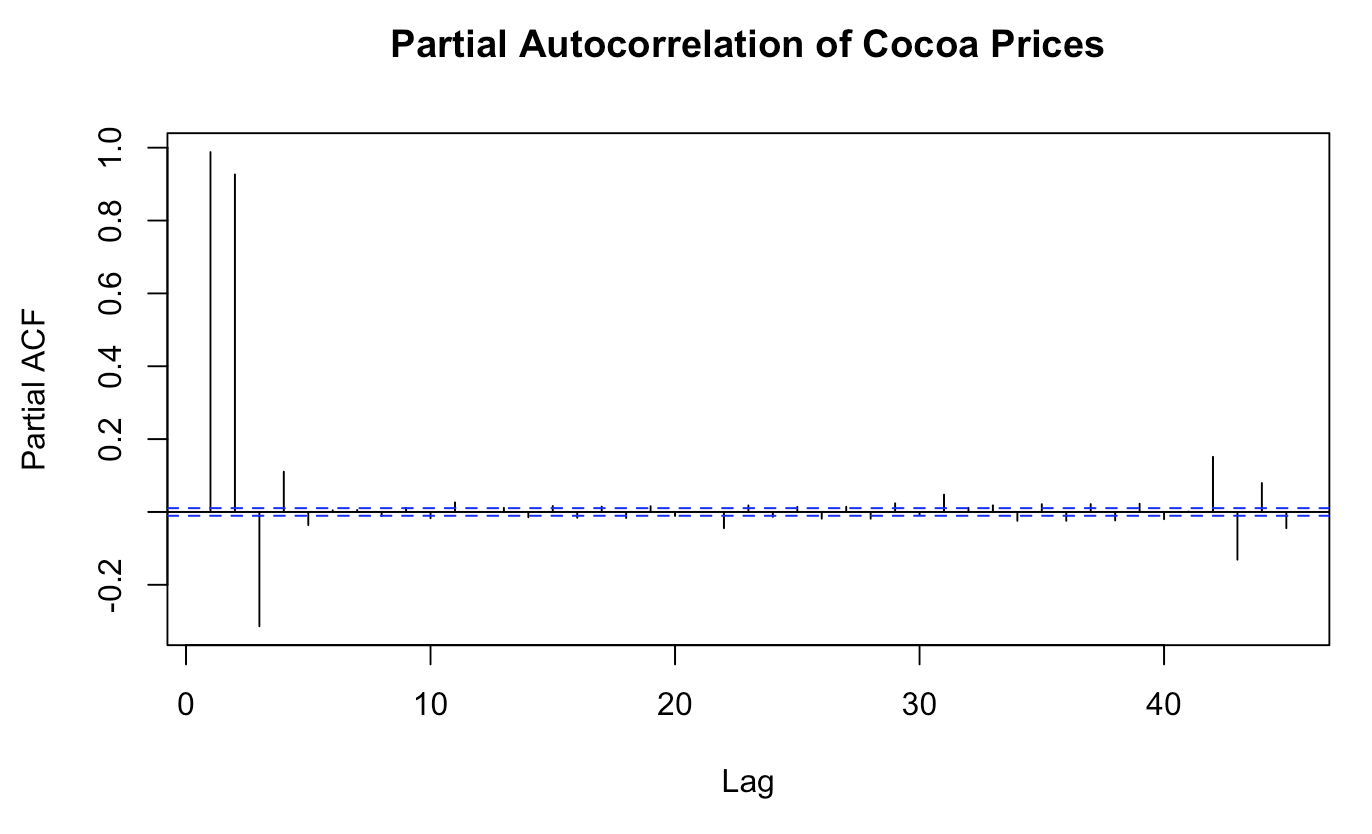
\includegraphics[scale=0.5]{figures/1.1.4.png}
    \caption{PACF of Cocoa Prices}
    \label{fig:chart_a}
\end{figure}


\section{Correlation \& Cross-Correlation Analysis}
The correlation matrix shows the pairwise correlation coefficients between numeric variables in the dataset, visualized using a heatmap. Comparing Cocoa Prices to temperature variables, it is evident cocoa prices have little to no correlation with temperature and precipitation. There seems to be slight negative correlation between precipitation and temperature variables, possibly due to periods of rain being cooler. Exploring the relationship between cocoa prices and rainfall further using an ACF plot, we see that most lags exceed the 95\% confidence bounds, indicating statistical significance. However, since most lags are uniformly distributed, there is no specific lag where rainfall is predictive of cocoa prices. Similarly, when exploring the relationship between cocoa prices and temperature, we see the same pattern. Both Cross-Correlation Plots show that temperature and rainfall are both statistically correlated with cocoa prices across all lags. While both plots exhibit consistent but weak correlation with cocoa prices and are deemed statistically significant, their maximum cross correlation is extremely low (~0.01 for rainfall and ~0.06 for temperature), indicating low practical significance. 
\begin{figure}[!ht]
    \centering
    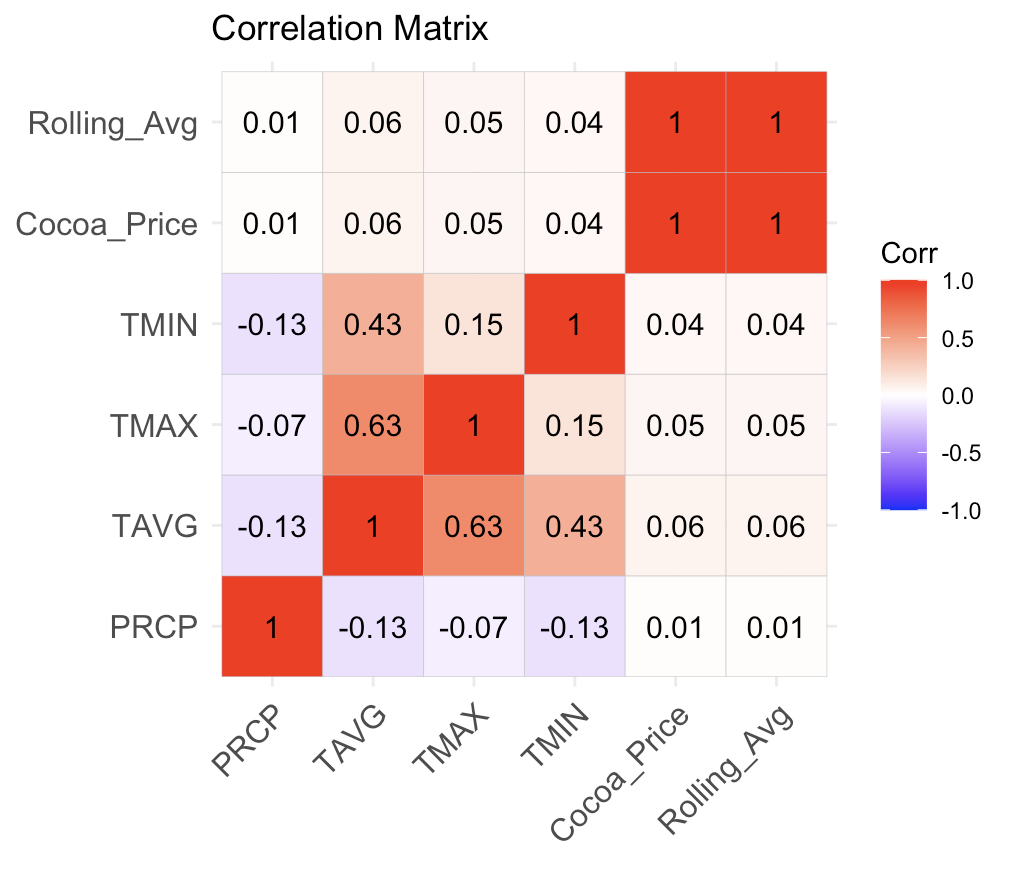
\includegraphics[scale=0.3]{figures/1.1.5.png}
    \caption{Correlation Matrix of Cocoa Prices vs. Temperature Variables}
    \label{fig:chart_a}
\end{figure}

\begin{figure}[!ht]
    \centering
    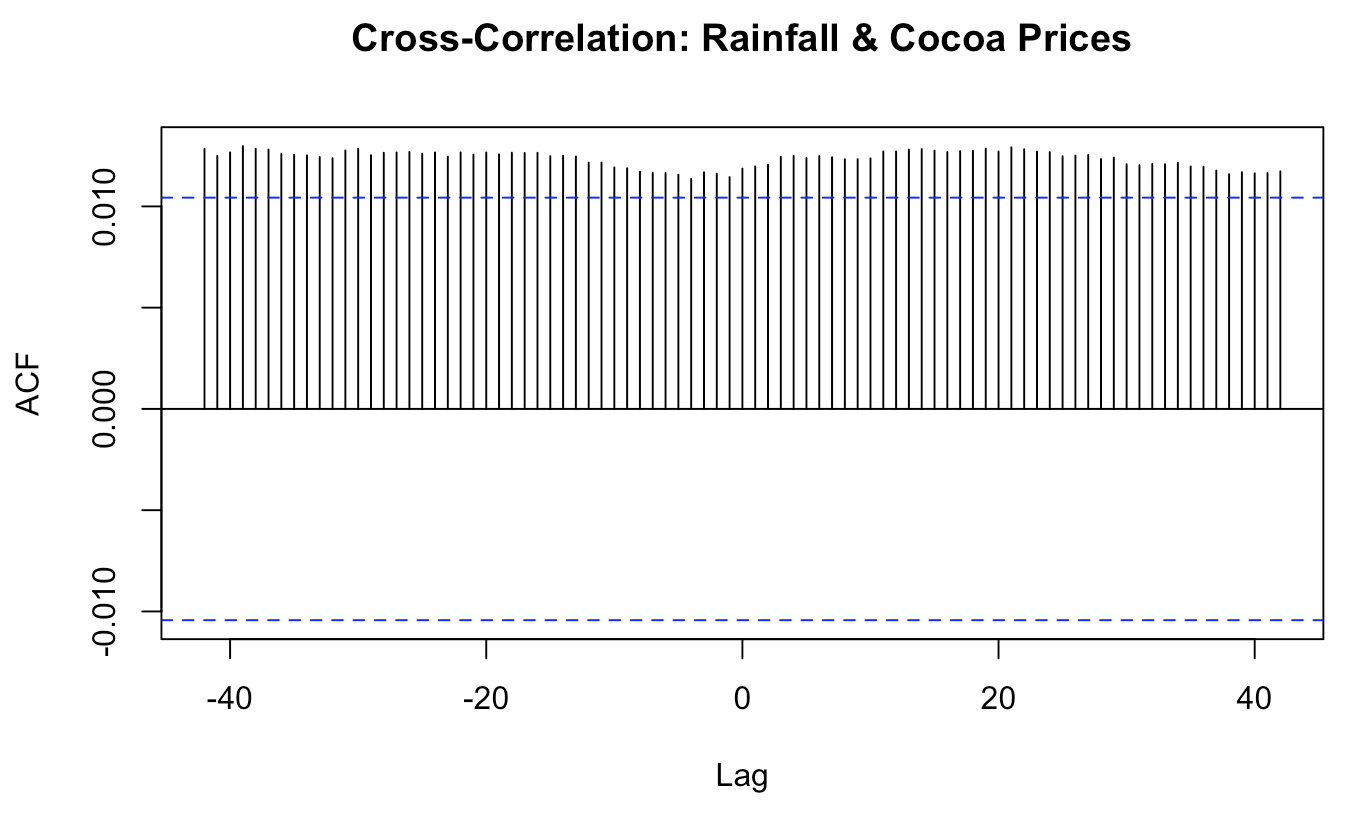
\includegraphics[scale=0.5]{figures/1.1.6.png}
    \caption{Cross-Correlation of Rainfall \& Cocoa Prices}
    \label{fig:chart_a}
\end{figure}

\begin{figure}[!ht]
    \centering
    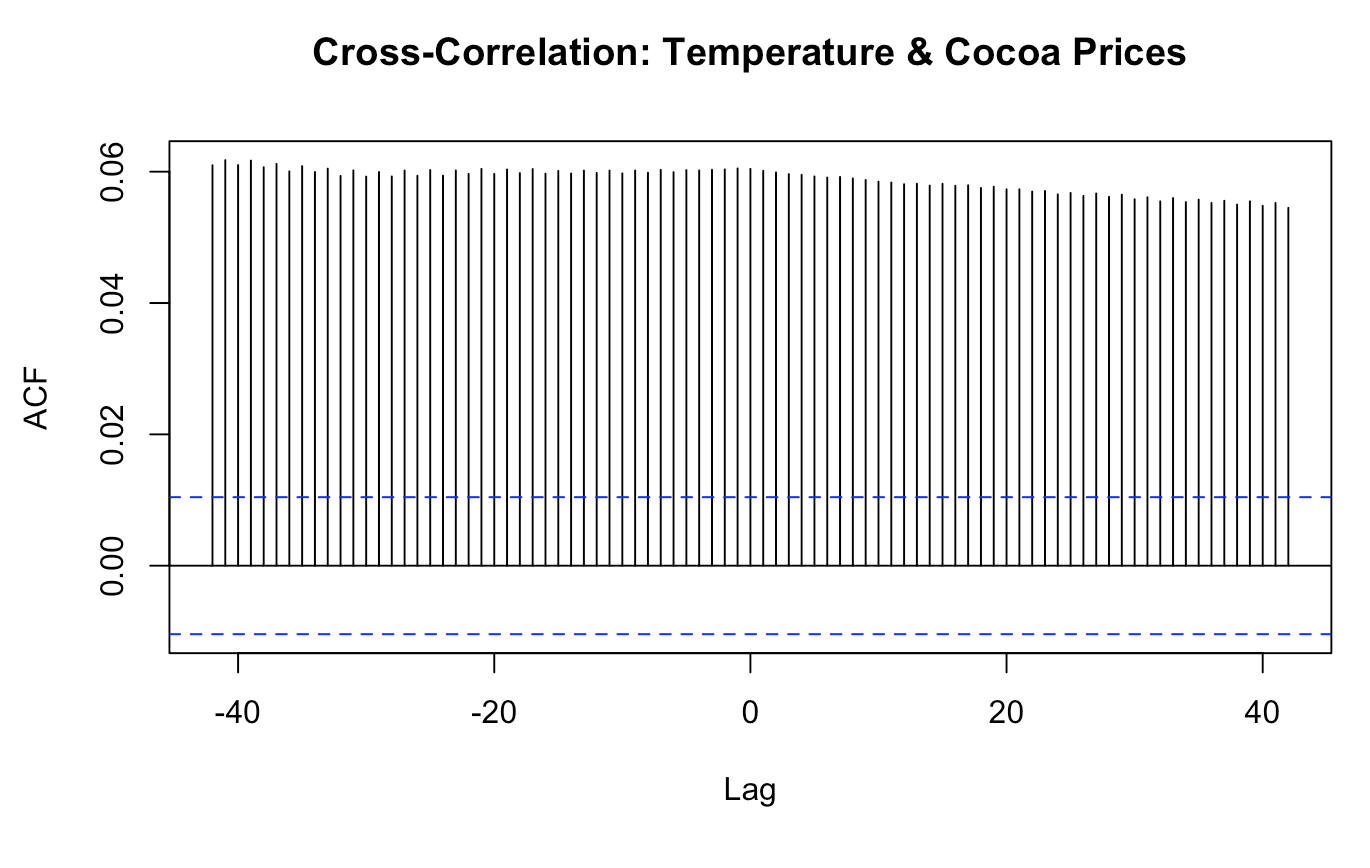
\includegraphics[scale=0.5]{figures/1.1.7.png}
    \caption{Cross-Correlation of Temperature \& Cocoa Prices}
    \label{fig:chart_a}
\end{figure}




\section{Log-Transformation \& Differencing}
To detrend/deasonalize the dataset, the dataset was log-transformed (red plot) and compared to the original time series (blue). While the log-transformation to stabilize variance, the dataset was still non-stationary, as evidenced by the upward spike near the end. To ensure non-stationarity of the log-transformed model, an Augmented Dickey Fuller (ADF) test is conducted with the alternative hypothesis that the series is stationary. The ADF reported a p-value of 0.6634, which fails to reject the null hypothesis that the log-transformed series is stationary. The log-transformed series is then differenced to achieve stationarity. Performing an ADF test on the log-differenced series reports a p-value of 0.01, accepting the alternative hypothesis that the series is now stationary.

\begin{figure}[!ht]
    \centering
    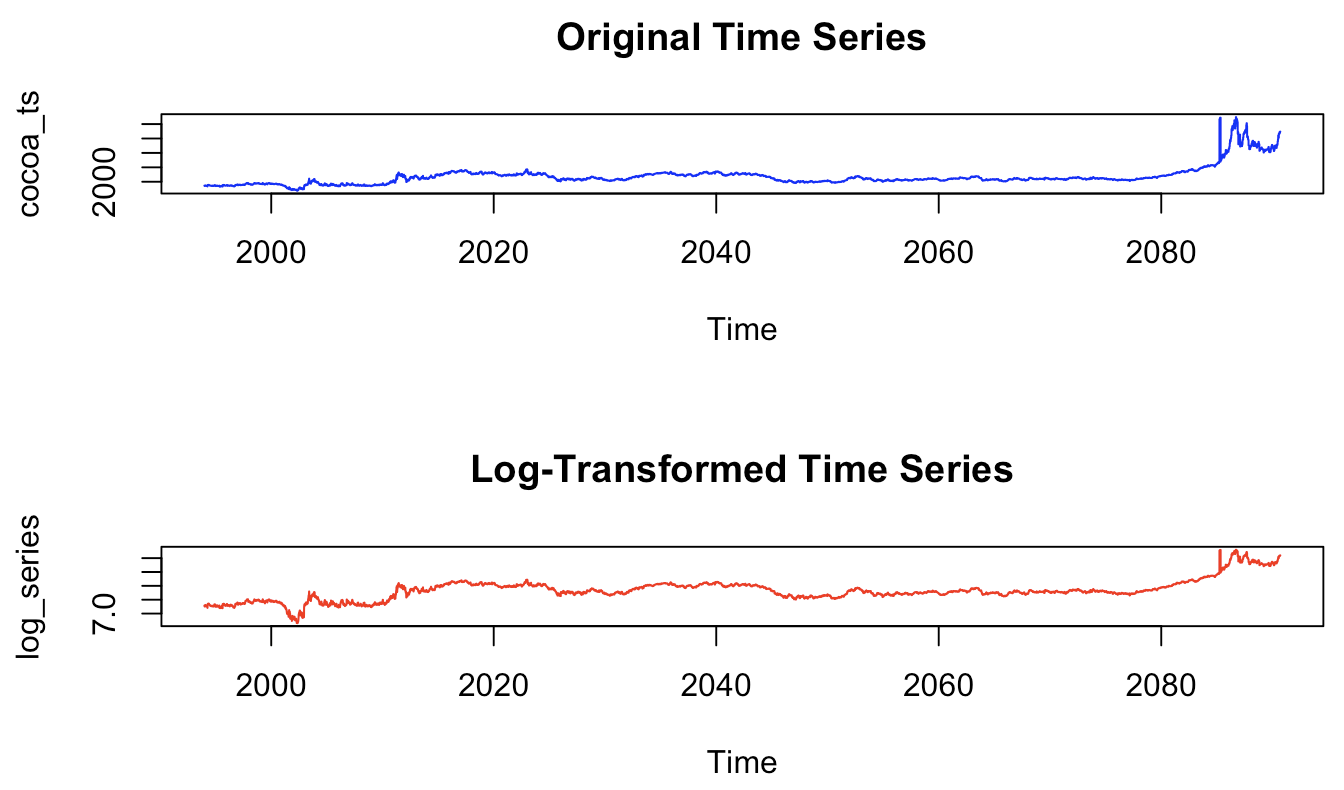
\includegraphics[scale=0.5]{figures/1.1.8.png}
    \caption{Log-Transformed Time Series}
    \label{fig:chart_a}
\end{figure}
\begin{figure}[!ht]
    \centering
    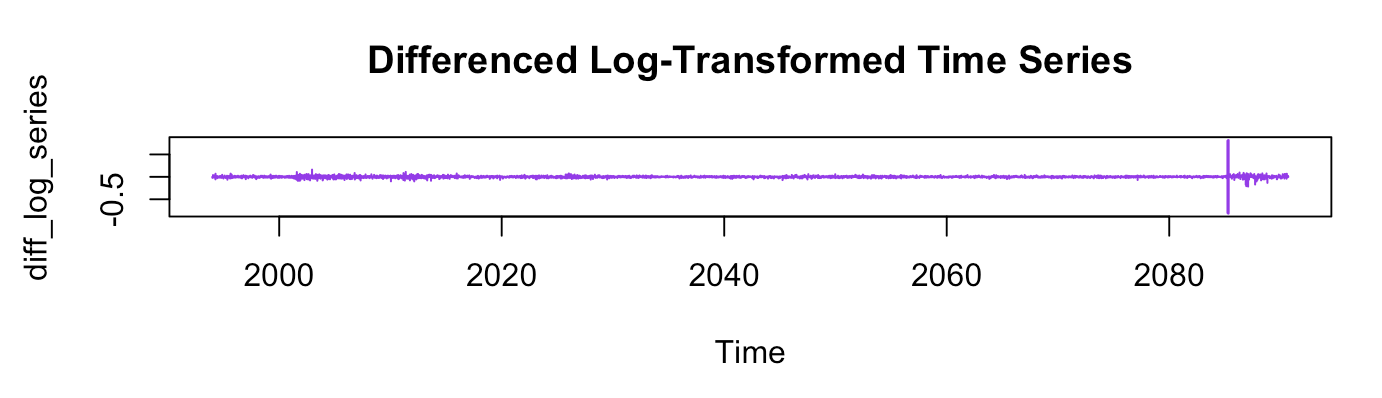
\includegraphics[scale=0.5]{figures/1.1.9.png}
    \caption{Differenced Log-Transformed Time Series}
    \label{fig:chart_a}
\end{figure}

\section{Model Building and Mathematical Formulation}
\textbf{Baseline ARIMA Selection}: \\
Multiple ARIMA models, including ARIMA(0,1,1), ARIMA(1,1,0), \- ARIMA(1,1,1), ARIMA(2,1,1), ARIMA(3,1,0), and \verb|auto.arima()|, were tested on a training subset of the cocoa price time series. Performance was validated on a 12-month test set using RMSE, MAE, and AIC. ARIMA(3,1,0) outperformed all others, showing the lowest RMSE and satisfying residual diagnostics (i.e., no autocorrelation, white noise residuals). It was therefore selected as the benchmark model.\\
\textbf{ARIMAX Extension}:\\
 To evaluate the predictive utility of external variables, we built ARIMAX(3,1,0) models incorporating:
\begin{itemize}
    \item \textbf{Climate Models}: AvgTemp and TotalRainfall (current and lagged)
    \item \textbf{Economic Models}: CPI and PPI (current and lagged)
\end{itemize}
Each dataset was split into a training (all but last 12 months) and testing (last 12 months) set. The external regressors were standardized and fed into the ARIMAX models using the \verb|forecast::Arima()| function.


\subsection{ARIMA Model Specification}

The general ARIMA$(p,d,q)$ model is defined as:

\begin{equation}
Y_t = c + \phi_1 Y_{t-1} + \phi_2 Y_{t-2} + \cdots + \phi_p Y_{t-p} + \theta_1 \epsilon_{t-1} + \cdots + \theta_q \epsilon_{t-q} + \epsilon_t
\end{equation}

where:
\begin{itemize}
    \item $Y_t$ is the differenced series after applying $d$ differencing operations.
    \item $\phi_i$ are the autoregressive (AR) coefficients.
    \item $\theta_j$ are the moving average (MA) coefficients.
    \item $\epsilon_t$ is white noise.
\end{itemize}

In our study, we selected the ARIMA(3,1,0) model based on forecast performance. This model implies:
\begin{itemize}
    \item $p = 3$ (three autoregressive terms),
    \item $d = 1$ (first differencing to remove trend),
    \item $q = 0$ (no moving average term).
\end{itemize}

\subsection{ARIMAX Model with External Variables}

To extend ARIMA by incorporating exogenous variables, we use the ARIMAX model. Its formulation is:

\begin{equation}
Y_t = c + \sum_{i=1}^{p} \phi_i Y_{t-i} + \sum_{j=1}^{k} \beta_j X_{j,t} + \epsilon_t
\end{equation}

where:
\begin{itemize}
    \item $X_{j,t}$ represents the $j$-th external regressor at time $t$ (e.g., CPI, PPI, AvgTemp),
    \item $\beta_j$ is the corresponding coefficient,
    \item Other terms as previously defined.
\end{itemize}

\subsection{Model Development Steps}
\begin{enumerate}
\item{Data Preparation}
\begin{itemize}
    \item Daily cocoa prices were aggregated to monthly averages ($\texttt{AvgPrice}$).
    \item Climate data were aggregated into:
        \begin{itemize}
            \item $\texttt{AvgTemp}$: Monthly average temperature,
            \item $\texttt{TotalRainfall}$: Monthly total precipitation.
        \end{itemize}
    \item Lagged variables were created:
        \begin{itemize}
            \item $\texttt{AvgTemp\_lag1}$, $\texttt{TotalRainfall\_lag1}$ (climate),
            \item $\texttt{CPI\_lag1}$, $\texttt{PPI\_lag1}$ (economics).
        \end{itemize}
\end{itemize}

\item{Model Training}
\begin{itemize}
    \item Time series was split with the last 12 months as test data.
    \item ARIMAX(3,1,0) ``Now'' models used $\texttt{CPI, PPI, AvgTemp, TotalRainfall}$
    \item ARIMAX(3,1,0) ``Lagged'' models used \texttt{CPI\_lag1, PPI\_lag1, AvgTemp\_lag1, TotalRainfall\_lag1}

\end{itemize}
\end{enumerate}

\subsection{Performance Metrics}

Models were evaluated using:
\begin{itemize}
    \item \textbf{RMSE}: Root Mean Square Error which penalizes larger errors.
    \item \textbf{AIC}: Akaike Information Criterion which balances model fit and complexity.
    \item \textbf{Ljung-Box Test}: Tests whether residuals are white noise.
\end{itemize}

\begin{table}[h!]
\centering
\caption{Model Performance Summary}
\begin{tabular}{lccc}
\toprule
\textbf{Model} & \textbf{AIC} & \textbf{RMSE} & \textbf{Ljung-Box $p$-value} \\
\midrule
Current Economic & 1771.59 & 1551.03 & 0.401 \\
Lagged Economic & 1843.32 & 2497.95 & 0.293 \\
Current Climate & 4286.36 & 3169.34 & 0.277 \\
Lagged Climate & 4285.77 & 3156.08 & 0.361 \\
\bottomrule
\end{tabular}
\end{table}

\subsection{Interpretation}

\begin{itemize}
    \item Economic models outperform climate models in forecasting cocoa prices.
    \item Current economic variables are more predictive than lagged ones, suggesting immediate demand-side impact.
    \item Climate variables improve with a one-month lag, consistent with supply-side delays in crop production.
    \item Ljung-Box results show no significant autocorrelation, confirming residuals are white noise.
\end{itemize}

\subsection{Conclusion}

The ARIMAX(3,1,0) model effectively captures both time-dependent structure and external shocks. Incorporating macroeconomic and climate variables improves forecasting accuracy, especially when lags are applied appropriately. The findings suggest demand-side shocks have immediate influence, while supply-side effects manifest with a lag—valuable insight for stakeholders planning around cocoa market volatility.